\documentclass{article}
\usepackage[utf8]{inputenc}

\documentclass[12pt,a4paper]{article}
\usepackage[top=0.70in, bottom=0.70in, left=0.8in,right=0.80in]{geometry} 
\usepackage[pdftex]{graphicx} 
\usepackage[bookmarks,  colorlinks=false]{hyperref}
\hypersetup{pdfborder = {0 0 0}}
\usepackage[final]{pdfpages} 
\usepackage{float} 
\usepackage{hyperref}
\usepackage{pslatex} 
\usepackage{array} 
\usepackage{setspace}
\usepackage{float}
\usepackage{enumerate}
\usepackage{longtable}
\usepackage[english]{babel}
\usepackage{amsmath}
\usepackage{pgfpages}
\usepackage[font=small,labelfont=bf]{caption}
\def\figurename{\textbf{Figure }}

\usepackage{listings}
\usepackage{color}

\definecolor{dkgreen}{rgb}{0,0.6,0}
\definecolor{gray}{rgb}{0.5,0.5,0.5}
\definecolor{mauve}{rgb}{0.58,0,0.82}
 

%For the header and footer
\usepackage{fancyhdr}
\fancypagestyle{plain}{%
%\fancyfoot[L]{\emph{Department of Computer Engineering, SHORT NAME OF COLLEGE, Pune}} % except the center
\fancyfoot[R]{\thepage}
\renewcommand{\headrulewidth}{0.4pt}
\renewcommand{\footrulewidth}{0.4pt}
}

\pagestyle{fancy}

\rhead{\emph{Query Quest - Edu}}

\fancyfoot[LO,LE]{\emph{}}
\cfoot{}
\fancyfoot[RO, RE]{\thepage}
\renewcommand{\headrulewidth}{0.4pt}
\renewcommand{\footrulewidth}{0.4pt}
%Page Border
% 




%GLOBAL SETTINGS OVER, DOCUMENT BEGINS
\begin{document}
\renewcommand\bibname{References}
\lhead{ }

%FROM HERE YOUR PAGES START GETTING ADDED
%\pgfpagesuselayout{boxed}
%\setlength{\parindent}{1cm}
% includes the cover page
%\pgfpagesuselayout{boxed}
%\newpage
\begin{center}
\thispagestyle{empty}
\Large{\textbf{A SEMINAR REPORT\\ \large{ON}}}\\[0.7cm]
\LARGE{\textsc {\textbf{``aaaa''}}}\\[0.5cm]
\vspace{0.5cm}
\Large{\textbf{\\Submitted to}}
\LARGE{\textbf{\\SAVITRIBAI PHULE PUNE UNIVERSITY\\}}
\vspace{1cm}
\Large{\textbf{\\In Partial Fulfilment of the Requirement for the Award of\\}}
\Large{\textbf{\\BACHELOR'S DEGREE IN\\COMPUTER ENGINEERING}}
\vspace{1cm}
\Large{\textbf{\\BY}}\\[0.5cm]
\begin{table}[h]
\centering
\Large{
\begin{tabular}{>{\bfseries}lc>{\bfseries}r}
NAME OF MEMBER  & & ROLL NUMBER A\\
\end{tabular}}
\end{table}
\vspace{0.5cm}
\large{\textbf{UNDER THE GUIDANCE OF}}\\
\large{\textbf{PROF. GUIDE NAME}}\\
\vspace{1cm}
\large{\textbf{DEPARTMENT OF MASTER OF COMPUTER APPLICATION}}\\
\Large{\textbf{TRINITY ACADEMY OF ENGINEERING}}\\
\large{\textbf{Kondwa Annex, Pune - 411048}}
\large{\textbf{\\2021-2022}}\\
\vspace{1cm}
\Large{\textbf{Nov-Dec 2021\\}}
\newpage
\end{center}
%\newpage

\newpage
\begin{center}
\thispagestyle{empty}
\Large{\textbf{A PROJECT BASED LEARNING REPORT \\ON}}\\[0.1cm]
\Large{\textsc {\textbf{``Query Quest - Edu
''}}}\\
\vspace{0.1cm}

\includegraphics[scale=.4]{uop-logo}\\
\Large{\textbf{\\Submitted to}}
\LARGE{\textbf{\\ SAVITRIBAI PHULE PUNE UNIVERSITY\\}}
\large{\textbf{\\In Partial Fulfilment of the Requirement for the Award of\\}}
\LARGE{\textbf{\\ SECOND YEAR IN MASTER OF COMPUTER APPLICATION}}
\vspace{0.3cm}
\Large{\textbf{\\BY}}\\[0.1cm]
\begin{table}[h]
\centering
\Large{
\begin{tabular}{>{\bfseries}lc>{\bfseries}r}
  Yash Rahul Bhande & & 5239\\
  
 
\end{tabular}}
\end{table}
\large{\textbf{UNDER THE GUIDANCE OF}}\\
\large{\textbf{ Mrs. Vibha Upadhaya}}\\[0.1cm]

\includegraphics[scale=0.3]{tae.png}\\
\large{\textbf{DEPARTMENT OF MASTER OF COMPUTER APPLICATION}}\\
\Large{\textbf{TRINITY ACADEMY OF ENGINEERING}}\\
\large{\textbf{Kondhwa Annex, Pune - 411048}}
\large{\textbf{\\2023-2024}}\\

%\Large{\textbf{NAME OF COLLEGE}}\\
%\large{\textbf{LOCATION IN PUNE, PUNE - PINCODE}}
%\large{\textbf{\\2021-2022}}\\[0.5cm]
%\Large{\textbf{AFFILIATED TO}}\\[0.5cm]
%
\includegraphics[scale=.5]{project/images/uop-logo}\\
%\LARGE{\textbf{UNIVERSITY OF PUNE}}
\newpage

\end{center}
\newpage

% includes the certificate page
\begin{center}
\thispagestyle{empty}

\LARGE{\textbf{TRINITY ACADEMY OF ENGINEERING}} \\ 
\large{\textbf{Department of Master of Computer Application}}\\


\includegraphics[scale=0.3]{tae.png}\\[1cm]

{\Huge \textbf{CERTIFICATE}}\\[0.5cm]
\end{center}
\linespread{1.13}
\large{\centering{This is certify that the Project Based Learning entitled}\\[0.2cm]
\textbf{\Large{\centering{``Query Quest - Edu``}}}\\[0.2cm]
\centering{submitted by}\\[0.2cm]
\begin{table}[h]
\centering
\large{
\begin{tabular}{>{\bfseries}lc>{\bfseries}r}
  Yash Rahul Bhande & & 5239\\

\end{tabular}}
\end{table}
This is to certify that \textbf{Yash Rahul Bhande (5239) } has successfully submitted Project Based Learning entitled  "\textbf{ Query Quest - Edu}" under the guidance of "\textbf{Mrs. Vibha Upadhay}" in the Academic Year 2023-24 at Master of Computer Application Department of Trinity Academy of Engineering , under the Savitribai Phule Pune University. This Project Based Learning  work is duly completed.}\\[0.5cm]
\large{\textbf{Date:15\hspace*{0.1cm}/03\hspace*{0.1cm}/2024}}\\
\vspace*{0.8cm}
\large{\textbf{Place: Pune}\\


\begin{spacing}{0}
\vspace{1.9cm}
\large{\textbf{(Mrs. Vibha Upadhay
)}}\hspace {1.3in}\large{\textbf{(Dr. A.A.Bhusari)}}\hspace*{1.3 in}\large{\textbf{(Dr. N. J. Uke)}}\\
\hspace*{0.6in}\textbf{PBL Guide}\hspace*{2.2in}\textbf{HOD} \hspace*{1.9in}\textbf{Principal}\\[10cm]
%\hspace*{0.3in}\large{\textbf{(Dr. N J Uke)}}\\
%\hspace*{0.4in}\textbf{Principal}
%\hspace*{2.5in}\textbf{External Examiner}\\[1.0cm]
\end{spacing}

 
%\newpage

% includes the acknowledgements page
\begin{center}
\thispagestyle{empty}
\LARGE{\textbf{Acknowledgements}}\\[1cm]
\end{center}
\linespread{1.13}
\large{\paragraph{}
I would like to acknowledge all the teacher and friends who ever helped and assisted me throughout my Project Based Learning  work.\newline \newline
First of all I would like to thank my respected guide \textbf {Mrs. Vibha Upadhay}, Introducing me throughout features needed. The time-to-time guidance, encouragement and valuable suggestion received from him are unforgettable in my life. This work would not have been possible without the enthusiastic response, insight and new idea from him.\newline \newline
Furthermore, I would like to thank respected \textbf{Dr. N. J. Uke}, Principal and  \textbf{Dr. A.A. Bhusari}, Head of Department of Master of Computer Application for the provided by him during my PROJECT BASED LEARNING work. I am also grateful to all the faculty members of Trinity Academy of Engineering, Pune for their support and cooperation. I would like to thank my lovely parent for time-to-time support and encouragement and valuable suggestion, and I would specify like to thank all my friends for their valuable suggestion and support. The acknowledgement world be incomplete without mention of the blessing of the almighty, which helped me in keeping high moral during difficult period.
}
\large{\paragraph{}

\begin{flushright}
{
\textbf {Yash Rahul Bhande}

}
\end{flushright}
\newpage
 
\newpage

\begin{center}
\thispagestyle{empty}
\vspace{2cm}
\LARGE{\textbf{ABSTRACT}}\\[1.0cm]
\end{center}
\thispagestyle{empty}
In today's fast-paced digital environment, the importance of accessible and engaging online learning platforms for learning facilitators cannot be underestimated. This content introduces "Query Quest - Edu", an interactive online learning program developed using HTML, CSS, JavaScript and PHP technologies.\newline

'Query Quest - Edu' stands as an educational beacon providing a variety of educational video content covering a wide range of topics including but not limited to coding, business, design, marketing, music, photography, software and science. Thanks to carefully designed playlists and seamless navigation, students have access to a variety of educational programs tailored to their personal interests and learning expectations.\newline

The spirit of "Query Quest - Edu" is based on the goal of encouraging curiosity, encouraging discovery and encouraging users to seek knowledge. By offering a recognized and user-friendly educational ecosystem, "Query Quest - Edu" actively promotes a culture of collaboration and collaboration, thus enabling deep and meaningful learning for students of all backgrounds and skill levels.\newline

The theme of the name "Query Quest - Edu" summarizes the platform's unwavering commitment to supporting curiosity-driven educational adventures. Based on a commitment to continuous improvement and innovation, "Query Quest - Edu" strives to become an online learning community that encourages students to participate in the changing world, learning science that holds the promise of discovery, inspiration and personal growth.\newline

This content provides a general introduction to the overall vision and principles of "Query Quest - Edu" regarding its immense potential to revolutionize online education and help students around the world.

 \vspace{0.5cm}


 % adds the Research Methodology page
\newpage


%TABLE OF CONTENTS AND LIST OF FIGURES ARE AUTOMATICALLY ADDED BY FOLLOWING COMMANDS
%ADD FIGURE OF TABLES IF YOU NEED TO, CHECK DOCUMENTATION
\pagenumbering{roman} %numbering before main content starts


%To reset the Header & Footer for TOC and LOF
\pagestyle{empty}
\addtocontents{toc}{\protect\thispagestyle{empty}}

\tableofcontents % adds Index Page 
\newpage
\listoffigures % adds List of Figures
\addtocontents{lof}{\protect\thispagestyle{empty}}
%\listoffigures % adds List of Figures
\cleardoublepage

%And reset back the settings we choose for Header and Footer
\pagestyle{fancy}

\newpage
\pagenumbering{arabic} %reset numbering to normal for the main content

\section{About Project }
\subsection{Title}
\paragraph{}The title of our project is \textbf{ “Query Quest-  Edu”}
\subsection{Domain}
\paragraph{}Online Education/E-Learning Platform
\subsection{Aim }
\paragraph{}Query Quest - Edu's overall goal is to disrupt the traditional education system to bridge the gap between students and provide access to quality education in the digital age. Query Quest - Edu is committed to providing free access to knowledge and helping people from diverse backgrounds begin educational transformation by creating a powerful and inclusive online platform.

\paragraph{}Query Quest - Edu specifically aims to achieve the following goals:

\begin{itemize}
\item Provide Usability: Query Quest - Edu aims to achieve this by providing an easily accessible online platform that can be accessed from anywhere, anytime. complete any educational program. The platform eliminates geographical and financial barriers, allowing international students to access quality educational content.

\item Encouraging Participation: The core of Query Quest - Edu's mission is to create a strong and interactive learning community. Through features such as curated playlists, user-generated content, and interactive learning modules, the platform encourages interaction and collaboration between students, fostering a culture of knowledge sharing and peer support.

\item Personalized Learning: Query Quest - Edu recognizes that each student is unique and therefore strives to provide personalized learning tailored to individual interests, preferences and standards. Leveraging data-driven insights and adaptive learning algorithms, the platform provides customized recommendations and learning methods to optimize each user's learning experience.

\item Supporting Lifelong Learning: Query Quest - Edu is committed to promoting a love of lifelong learning by providing a variety of courses that meet the needs of students of all ages, ages and skill levels. Constantly expanding and constantly updating its content library, the platform aims to arouse curiosity in users, encourage intellectual curiosity and stimulate brain development.
\end{itemize} 
More importantly, Query Quest - Edu wants to be more than just an online education; It aims to be a social change, helping people realize their potential, find their interests and create a future for themselves and future generations. in the future.

\newpage


\subsection{Objective}
\begin{itemize}
\item Enhanced Accessibility: Query Quest - Edu aims to provide quality education to a wide range of students regardless of location, economic status or physical limitations. By providing an online platform that can be accessed from any internet device, the aim is to make the courses accessible to everyone with an internet connection.

\item Encouraging Collaboration: Query Quest - Edu is committed to fostering collaboration by providing interactive learning experiences, collaboration tools, and community forums to enable collaboration with users. The goal is to create a strong learning community where students can connect with their peers, share knowledge, and collaborate on projects.

\item Personalized Learning: Query Quest - Edu is committed to providing personalized learning to all users based on their personal interests, preferences and learning styles. By analyzing data and machine learning algorithms, the aim is to provide appropriate recommendations, learning modifications and personalized recommendations to improve the learning experience.

\item Promoting lifelong learning: Query Quest - Edu aims to foster a culture of lifelong learning by providing a variety of educational content that meets the needs of students of all ages and skill levels. The goal is to spark curiosity, encourage intellectual development, and encourage a love of learning that goes beyond art.

\item Empowering Educators: Query Quest - Edu recognizes the critical role of educators in enhancing learning and aims to empower them with tools, resources and development efforts. The aim is to support teachers in creating an engaging and effective learning experience for students, ultimately improving the quality of learning through the platform.
   
\end{itemize} 
\newpage
\subsection{Problem Statement }

\paragraph{} The education system is currently grappling with issues that impede access to quality education and hinder international students' learning. These issues include:
\begin{itemize}
\item Limited Access: Many people, especially those living in remote or underserved areas, cannot access quality education due to geographic restrictions, usage restrictions, or financial constraints. This lack of education leads to educational inequality and widens the gap between the privileged and the poor.

\item Engagement Issues: Traditional education systems often disable students, leaving them less engaged, less engaged, and less motivated. Exaggerated learning, exaggerated curriculum, and lack of interactive learning can make students disinterested and inhibit the development of positive thinking.

\item One-size-fits-all approach: Traditional education systems follow a standard, one-size-fits-all approach. -A one-size-fits-all approach fails to meet the student's diverse learning needs, preferences, and abilities. This integrated approach does not accommodate different learning styles, challenges, and interests, resulting in a learning environment that may not meet the needs of all students.

\item Teacher Support: Teachers often struggle to convey knowledge, self-manage, provide timely feedback, and meet students' individual needs. The girl in the older class. Limited resources, high teacher-student ratios, and inadequate infrastructure can inhibit teacher effectiveness and impact student learning.

\item There is no way to learn forever: The main focus of technical education is the transfer of knowledge and skills within a limited period of time. Pioneers often overlook the importance of continuous learning and skill development. As a result, people will have difficulty adapting to rapid changes in the market, technological changes and changing social needs, and the work they do will become good and useless.
\end{itemize} 

 \paragraph{}According to these challenges, there is an urgent need for new solutions that use technology, personal learning and the integration of the learning environment to meet the different needs of students and teachers. Query Quest - Edu strives to solve these problems by providing an accessible, engaging and personalized online learning platform that enables students to realize their potential and pursue lifelong learning.




 % adds the introduction page
\newpage
\section{Introduction}

\subsection{Introduction}

In today's rapid development, the educational environment has transformed into online learning platforms. In this transition, Query Quest - Edu serves as a beacon of innovation poised to transform the way we teach. With its user-friendly interface and many educational features, Query Quest - Edu strives to provide free access to knowledge and empower students worldwide. This introduction sets the stage for exploring the evolution of Query Quest - Edu and highlights its commitment to encouraging curiosity, encouraging engagement, and fostering lifelong learning. Join us on our journey to discover the endless possibilities of learning at Query Quest - Edu.



\subsection{Project Introduction}
Welcome to Query Quest - Edu, where education meets innovation! Query Quest - Edu is not just another online learning platform; It is a wonderful learning center designed to inspire and engage students every day. Query Quest - Edu aims to revolutionize education with its design and interactive features. This brief project provides an overview of Query Quest - Edu's goals, capabilities, and key motivations driving its growth. Query Quest - Edu is committed to helping students realize their potential and succeed in their academic careers by integrating technology, creativity and expertise. Join us on an exciting journey of discovery and growth with Query Quest - Edu.

\subsection{Project Scope}
Query Quest - Edu aims to create an online learning platform that meets the needs of global students. The working of the program covers many important aspects required to create a good learning ecosystem. First, Query Quest - Edu will provide a wide range of educational content across a variety of disciplines, including careers, business, design, business, music, photography, software and science. This rich library provides students with access to resources tailored to their interests and learning goals. Secondly, the platform will prioritize user experience with a user-friendly interface and intuitive navigation. Interactive content such as quizzes, forums and live meetings will be integrated to stimulate and stimulate learning. Third, Query Quest - Edu will provide personalized learning through customized learning, recommendation algorithms, and bookmarking functions. This personalized program is designed to meet individual learning preferences and adapt to each student's unique needs. Finally, the platform will prioritize accessibility and scalability, ensuring that educational resources are accessible to all users and able to accommodate growth and future expansion. By addressing these basic concepts, Query Quest - Edu aims to help students meet their educational needs and unlock their full potential.

\newpage









\newpage

\section{Literature Survey}
\subsection{Literature Survey}
\paragraph{}Query Quest - Edu's research database provides research, publications and research related to online education, app design, personalized learning and access to education. The purpose of this chapter is to provide an overview of the current state of online education and to identify the main issues, challenges and opportunities related to the development of Query Quest - Edu.


\paragraph{}The literature review will examine the following topics: 

\begin{itemize}
\item Online Learning Platforms: A study of existing online learning platforms and their features, performance and effectiveness of educational support.

\item User Experience Design: Learn about user interface design principles, usability, and user experience design in online learning.

\item Personalized Learning: Identification of personalized learning strategies, emerging learning technologies and their effects on student motivation, participation and learning.

\item Accessibility in Education: Explore accessibility standards, guidelines, and best practices for creating online education for people with disabilities.
\end{itemize} 

\paragraph{}Through the results of comprehensive data analysis, Query Quest - Edu aims to gain insight, inform design decisions and identify areas for development, innovation and development to create user-friendly, efficient and inclusive online learning platforms.



\subsection{Conclusion}
\paragraph{}Case studies demonstrate the diversity of online learning platforms and highlight the importance of user-friendly design, personalized learning and accessibility. Insights from existing studies guide the development of Query Quest - Edu, ensuring that user involvement, identity, and engagement are important. Query Quest - Edu aims to use these findings to create a new online education that meets the needs of global students, encouraging motivation, memory and learning, and well-being in a practical and productive environment.

.

\vspace{9.5cm}




 % adds the Literature Survey page

\newpage
%\input{project/req-analysis.tex}
%\section{System Design}
\section{SECTION NAME}
\paragraph{} WRITE HERE.
\newpage
% %  \section{ Software Requirements Specification  }
% % \subsection{Functional Requirement}
% % \subsubsection{System Feature:}
% % 1. Asset Registration: Users can input details of newly acquired assets into the system.\newline
% % 2. Asset Tracking: Real-time tracking of asset location and movement within the organization.\newline
% % 3. Audit Trail: Maintaining a transparent log of all asset-related transactions and activities.\newline
% % 4. Maintenance Ticket Generation: Capability to create tickets for assets requiring servicing.\newline
% % 5. Returnable Gatepass: Handling the issuance and tracking of gatepasses for asset movements.\newline
% % 6. Order Management: Facilitating the process of ordering new assets or maintenance supplies.\newline



% % \subsection{External Interface Requirement: }

% % \subsubsection{Hardware Interface:}

% % 1. Mobile Devices: The mobile app is compatible with iOS and Android devices.\newline
% % 2. Internet Connectivity: Requires stable internet access for real-time updates.\newline

% % \subsubsection{Software Interface:}
% % 1. Compatibility: Integration with backend databases and servers for data synchronization.\newline
% % 2. User Authentication: Integration with secure user authentication systems.\newline

% % \subsection{System Requirement:}
% % \subsubsection{Database Requirement:}
% %  1. SQLite 
% % \subsubsection{Software Requirement:}

% % 1. Android Studio \newline
% % 2. Any version of internet exlporer.\newline
% % 3. Visual studio.\newline
% % 4. Android SDK\newline
% % 5. JAVA JDK\newline

% % \subsubsection{Hardware Requirement:}
% % 1. Smart Phone \newline
% % 2. Android Version\newline
% % 3. 4GB RAM
% % \newpage
% %  \subsection{Analysis Model}
% %  \subsubsection{System Life Cycle}
% %  \begin{figure}[H]
% %   \centering
% %   \includegraphics[scale=0.4]{astl1.png}    \caption{\textbf{ Model}}
% % \end{figure}

% % Your previous LaTeX content here...

% \subsection{Analysis Model}
% \subsubsection{System Life Cycle}
% \begin{figure}[H]
%   \centering
%   \includegraphics[scale=0.4]{astl1.png}
%   \caption{\textbf{Model}}
% \end{figure}

% \section{Software Requirements Specification}
% \subsection{Functional Requirement}
% \subsubsection{System Feature:}
% 1. Asset Registration: Users can input details of newly acquired assets into the system.\newline
% 2. Asset Tracking: Real-time tracking of asset location and movement within the organization.\newline
% 3. Audit Trail: Maintaining a transparent log of all asset-related transactions and activities.\newline
% 4. Maintenance Ticket Generation: Capability to create tickets for assets requiring servicing.\newline
% 5. Returnable Gatepass: Handling the issuance and tracking of gatepasses for asset movements.\newline
% 6. Order Management: Facilitating the process of ordering new assets or maintenance supplies.\newline

% \subsection{External Interface Requirement: }
% \subsubsection{Hardware Interface:}
% 1. Mobile Devices: The mobile app is compatible with iOS and Android devices.\newline
% 2. Internet Connectivity: Requires stable internet access for real-time updates.\newline

% \subsubsection{Software Interface:}
% 1. Compatibility: Integration with backend databases and servers for data synchronization.\newline
% 2. User Authentication: Integration with secure user authentication systems.\newline

% \subsection{System Requirement:}
% \subsubsection{Database Requirement:}
% 1. SQLite 
% \subsubsection{Software Requirement:}
% 1. Android Studio \newline
% 2. Any version of Internet Explorer.\newline
% 3. Visual Studio.\newline
% 4. Android SDK\newline
% 5. JAVA JDK\newline

% \subsubsection{Hardware Requirement:}
% 1. Smart Phone \newline
% 2. Android Version\newline
% 3. 4GB RAM



% \newpage
% % New text insertion
% % \subsection{Analysis Model Continued}
% % \subsubsection{System Life Cycle (Continued)}
% % \begin{figure}[H]
% %   \centering
% %   \includegraphics[scale=0.2]{astl1.png}
% %   \caption{\textbf{Model}}
% % \end{figure}
% % \vspace{2cm}
% % \item 1. Supervisor's room: This is where the supervisor can monitor and manage the entire warehouse operation.\newline
% % \item 2. Main warehouse: This is where the physical goods are stored.\newline
% % \item 3. Cloud database: This is where all of the warehouse data is stored, such as inventory levels, location of goods, and order information.\newline

% \subsection{Analysis Model Continued}
% \subsubsection{System Life Cycle (Continued)}
% \begin{figure}[H]
%   \centering
%   \includegraphics[scale=0.3]{astl1.png}
%   \caption{\textbf{Model}}
% \end{figure}

% \vspace{2cm}

% \begin{enumerate}
%   \item Supervisor's room: This is where the supervisor can monitor and manage the entire warehouse operation.
%   \item Main warehouse: This is where the physical goods are stored.
%   \item Cloud database: This is where all of the warehouse data is stored, such as inventory levels, location of goods, and order information.
% \end{enumerate}


% \newpage




% \subsection{Analysis Model}
% \subsubsection{System Life Cycle}
% \begin{figure}[H]
%   \centering
%   \includegraphics[scale=0.4]{astl1.png}
%   \caption{\textbf{Model}}
  
% \end{figure}
\newpage
\section{Software Requirements Specification}
\subsection{Functional Requirement}
\subsubsection{System Feature:}

\begin{itemize}
\item User registration and access: Users can access the features and content of the Platform by creating an account.

\item Search and search content: Users can search a wide variety of educational content, including topics such as coding, business, design, business, music, photography, software and science.

\item Create and manage playlists: Users can create custom playlists of educational videos to organize and save content for future use.

\item Interactive Tools: Query Quest - Edu offers interactive tools such as quizzes, forums and live meetings with teachers to enhance learning, collaborate and encourage learning.


\item Bookmark and save favorites: Users can bookmark their favorite content for easy access and save it to track their progress across different courses and playlists.
\end{itemize}

\subsection{External Interface Requirement:}
\subsubsection{Hardware Interface:}
\begin{itemize}
    \item 

\item Device compatibility: Query Quest - Edu can be accessed via compatible devices such as desktops, laptops, tablets and smartphones.

\item Internet connection: Users must have a stable Internet connection to access Query Quest - Edu and its features without any problems.

\item Dimensions and resolutions: The platform is designed to accommodate a variety of sizes and resolutions, ensuring visibility and usability on different devices.

\item Input devices: Query Quest - Edu supports compatible devices such as keyboards, mice, touch screens and digital pens for navigation and interaction.

\item Audio output: Users will need audio output capability (such as speakers or headphones) to listen to video lectures, discussions, and other content. multimedia message.

\item Camera (optional): Some features (such as Live chat or video conferencing) may require a built-in or other camera to participate.
\end{itemize}

\newpage


\subsection{System Requirement:}
\subsubsection{Database Requirement:}
\begin{itemize}
    

\item MySQL database management system
\end{itemize}

\subsubsection{Software Requirement:}
\begin{itemize}

\item Visual Studio Code (VSCode)
\item Web browser (e.g., Google Chrome, Mozilla Firefox)
\item XAMPP with PHP and MySQL

\end{itemize}

\subsubsection{Hardware Requirement:}
\paragraph{} For Computers:

\begin{itemize}
\item Desktop computer or laptop
\item Minimum 4GB RAM
\item Processor: Intel Core i3 or equivalent
\item Storage: At least 256GB SSD or HDD
\item Display: Monitor with a resolution of 1366x768 pixels or higher
\item Internet connectivity: Ethernet or Wi-Fi connection
\end{itemize}

\paragraph{} For Phones:

\begin{itemize}
\item Smartphone (Android or iOS)
\item Minimum 2GB RAM
\item Storage: At least 32GB internal storage
\item Processor: Qualcomm Snapdragon 600 series or equivalent for Android devices; Apple A10 Fusion or equivalent for iOS devices
\item Display: Screen size of at least 5 inches with a resolution of 720x1280 pixels or higher
\item Internet connectivity: Wi-Fi or mobile data connection
\end{itemize}
\newpage


\subsection{Analysis Model Continued}



\subsubsection{System Life Cycle (Continued)}


% \begin{figure}[H]
%   \centering
%   \includegraphics[scale=0.3]{astl1.png}
%   \caption{\textbf{Model}}
% \end{figure}

% \vspace{0.5cm}

% \begin{enumerate}
%   \item Supervisor's room: This is where the supervisor can monitor and manage the entire warehouse operation.
%   \item Main warehouse: This is where the physical goods are stored.
%   \item Cloud database: This is where all of the warehouse data is stored, such as inventory levels, location of goods, and order information.
% \end{enumerate}
\newpage

\newpage

\section{System Study and Analysis }

\subsection{Existing System }
\paragraph{}Current online learning systems are often built on fragmented data distributed across multiple platforms and locations. Students often face difficulties accessing general education content. They may need to browse multiple websites, apps, or physical resources to find relevant information, resulting in inconsistent learning. Additionally, the current system may not have interactive, self-selecting, and immediate feedback strategies, which may limit the effectiveness of the learning process. Overall, the current system may not be able to meet the changing needs and expectations of students in terms of accessibility, participation and flexibility in personal learning styles.

\subsection{Proposed System}
\paragraph{}The proposed system, Query Quest - Edu, aims to transform the current online education system by providing simple and comprehensive learning. Query Quest - Edu will provide a central place where users can access different educational content, unlike the resources of the current system. The platform will include a variety of content that will allow students to access resources based on their interests and learning goals. Focusing on user interaction and integration, Query Quest - Edu will provide interactive and practical options to enhance learning for all users. Through personalized recommendations and appropriate design, Query Quest - Edu aims to help students take control of their learning and realize their full potential.

\subsection{Feasibility System}
\paragraph{}Query Quest - Edu's study on the feasibility and effectiveness of implementing the planning process. It takes into account many factors such as work, work and productivity to determine efficiency and sustainability.

\begin{itemize}
    

\item Technical Feasibility: This aspect evaluates whether the proposed process can be developed using existing tools and resources. It evaluates features such as compatibility between software tools, data management, and programming languages needed for development. Additionally, technical feasibility checks the scalability and performance of the system to meet future growth and user needs.

\item Economic Feasibility: Economic feasibility analyzes the cost effectiveness of the design and management of the planning process. It takes into account things like construction costs, hardware and software costs, operating costs, and capital gains. Business feasibility also examines the project's return on investment (ROI) and financial value over time.

\item Operational Feasibility: Operational Feasibility measures the effectiveness of using the proposed system in an organization or user community. It considers factors such as user acceptance, training needs, operational planning, and potential impact on existing operations and processes. Functionality also measures the ease of maintaining, updating, and supporting a system on an ongoing basis.
\end{itemize}

\paragraph{}This research provides information on the technical, economic and operational aspects of the project, ultimately contributing to the success and long-term sustainability of the project.


\newpage


















\section{Data Flow }
% \begin{figure}[h!]
%     \centering
%      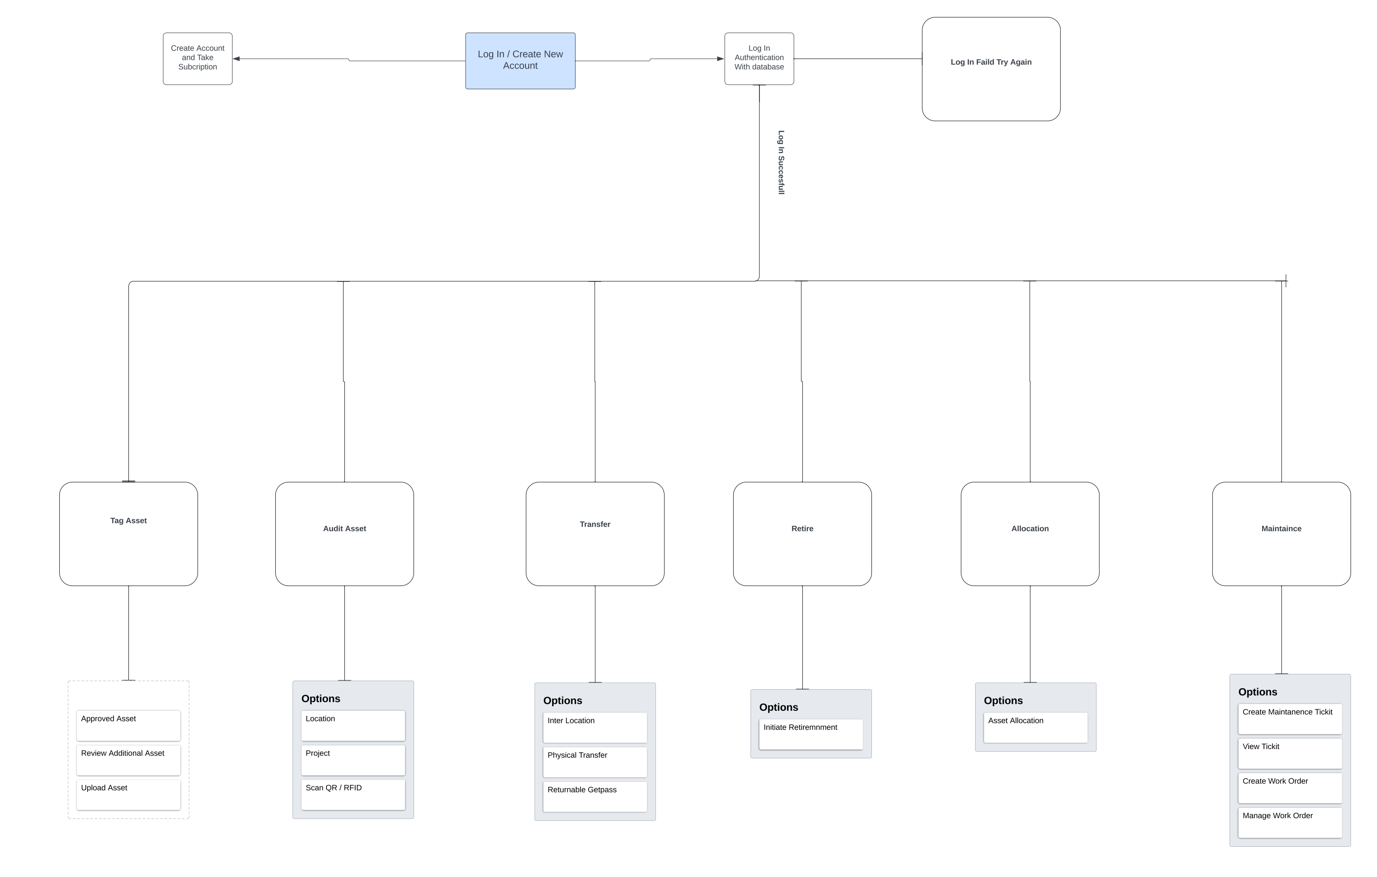
\includegraphics[scale=0.6]{save.png}  
% \end{figure}


% % New text insertion after the figure
% The diagram appears to show a high-level overview of a cloud-based warehouse management system (WMS). The main components of the system include a supervisor's room, a main warehouse, a cloud database, individual warehouses, RFID readers, mobile apps, and information sharing. The system uses RFID readers to track the location of goods in the warehouse, and this information is stored in the cloud database. The supervisor can use the information in the cloud database to monitor the warehouse operation and make sure that it is running smoothly. The system can be used to improve the efficiency and accuracy of warehouse operations.





% \newpage










\section{System Design }
% \subsection{File Upload Page}
% \begin{figure}[h!]
%     \centering
%     \includegraphics[scale=0.4]{uplodede.png}  
%      \caption{\textbf{Upload Page (Before Asset File Upload)}}
% \end{figure}

% \begin{figure}[h!]
%     \centering
%     \includegraphics[scale=0.4]{uploded.png}  
%      \caption{\textbf{Upload Page (After Asset File Upload)}}
% \end{figure}
% \vspace{0.5cm}

% \begin{enumerate}
%   \item Its an asset file upload page(Excel File).
%   \item Here user upload a assets with their description in the form of columns, the user can map a their file columns and columns inside a tables to add all upload all assets in bulk.
% \end{enumerate}

% \newpage
% \subsection{Home Page}
% \begin{figure}[h!]
%     \centering
%     \includegraphics[scale=0.4]{1 (1).jpeg}  
%      \caption{\textbf{Home Page}}
% \end{figure}

% \vspace{0.5cm}

% \begin{enumerate}
%   \item It's a home page of our mobile application and its contains a various buttons  to access all components for asset tracking.
%   \item Some examples of buttons like Tag asset gives access to asset tagging component, Transfer buttons Gives access to Transfer Asset Component etc
% \end{enumerate}
% \newpage
% \subsection{Topic}
% \begin{figure}[h!]
%     \centering
%      \includegraphics[scale=0.4]{1 (2).jpeg} 
%      \caption{\textbf{Asset Tagging Page}}
% \end{figure}
% \vspace{0.5cm}

% \begin{enumerate}
%   \item Its an asset tagging component,Used for tagging of asset.
%   \item In this component we can upload photo and also we can scan the asset for its tagging.
% \end{enumerate}
% \newpage
% \subsection{Topic}
% \begin{figure}[h!]
%     \centering
%      \includegraphics[scale=0.4]{transfer.jpeg} 
%       \caption{\textbf{Transfer Page}}
% \end{figure}
% \vspace{0.5cm}

% \begin{enumerate}
%   \item Transfer page is to track the location of asset.
%   \item Using this component we can track the asset like we can see the exact location of asset, we can check is this asset inside the organization or someone use this asset from home for WFH.
% \end{enumerate}
% \newpage
% \subsection{Topic}
% \begin{figure}[h!]
%     \centering
%      \includegraphics[scale=0.4]{audit.jpeg} 
%       \caption{\textbf{Audit Page}}
% \end{figure}
% \vspace{0.5cm}

% \begin{enumerate}
%   \item Using audit component we check the assets used by the branch and project.
%   \item On this component we see the total summary of assets used in particular project and location.
% \end{enumerate}
% \newpage
% \subsection{Topic}
% \begin{figure}[h!]
%     \centering
%      \includegraphics[scale=0.4]{retire.jpeg} 
%       \caption{\textbf{Retire Page}}
% \end{figure}
% \vspace{0.5cm}

% \begin{enumerate}
%   \item Using the retire component we check the life of asset and we can generate its retirement ticket.
%   \item Here we can add a retirement status to known the process of retirement.
% \end{enumerate}
% \newpage

% \subsection{Topic}
% \begin{figure}[h!]
%     \centering
%      \includegraphics[scale=0.4]{1 (5).jpeg} 
%       \caption{\textbf{Allocation Page}}
% \end{figure}
% \vspace{0.5cm}

% \begin{enumerate}
%   \item Using this allocation component we can allocate the asset to any person or project.
%   \item After the allocation we check the is we need to transfer this asset or not.
% \end{enumerate}
 
% \newpage
% \subsection{Topic}

% \begin{figure}[h!]
%     \centering
%      \includegraphics[scale=0.4]{1 (9).jpeg}
%       \caption{\textbf{Maintenance Page}}
% \end{figure}
%  \vspace{0.5cm}

% \begin{enumerate}
%   \item In this maintenance component we add a all feature to  the maintenance of asset.
%   \item In that we create a Maintenance Ticket, View created ticket,Create work order and manage work order.
% \end{enumerate}




%\input{project/implementation.tex} % adds the Project Design
%\input{project/screenshots.tex}
\newpage
\section{Conclusion}
\paragraph{} In summary, Query Quest - Edu represents a significant step forward in online education by providing a revolutionary platform designed to enhance the learning of users worldwide. Our main goal throughout the development of Questions Quest - Edu is to create a user-friendly, accessible and engaging environment that allows students to explore, discover and grow.

\paragraph{} Focusing on multiple learning, Query Quest - Edu provides users with a comprehensive knowledge base, discipline and discipline by eliminating barriers to accessing quality education. Quest Quest - Edu caters to students' diverse needs and interests by providing personalized learning opportunities, interactive tools, and accessible features to ensure education remains inclusive and accessible for all.

\paragraph{} In addition, the research conducted for the Query Quest - Edu project reveals the success and sustainability potential of the project. Through a rigorous analysis of skills, job and business, we identified opportunities for optimization and improvement to ensure Query Quest - Edu evolves according to change needs and learning challenges.

\paragraph{} As we look to the future, we think Query Quest - Edu is more than online education. It is a catalyst for change, a beacon of innovation and a driver of quality education. Query Quest - Edu has the potential to transform the way we learn, connect and interact with information by harnessing the power of technology, collaboration and creativity.

\paragraph{} Finally, we would like to thank everyone who has helped us, from the dedicated staff who work tirelessly behind the scenes to the users who have provided valuable advice and support and contributed to the development of Quest Quest - Edu. Query Quest - We embark on a journey of discovery, research and development together, using the endless resources provided by Edu. % adds the Scheduling and Planning page
\newpage

% \section{References}
% \begin{itemize}

%     \item American Management Association. (2018). Best Practices in Asset Management. Retrieved from \url{https://www.amanet.org/assets/1/6/AMA-quarterly-fall-18.pdf}
    
%     \item Johnson, R. (2020). Innovations in Asset Tracking: A Comprehensive Review. Journal of Inventory Management, 15(3), 45-58.
    
%     \item Smith, J. (2019). Efficient Inventory Control Techniques. ABC Publishing.
    
%     \item Asset Control Solutions. (2021). Annual Report on Asset Management Systems.
    
%     \item Brown, A. (2017). Optimizing Asset Utilization in Modern Organizations. Asset Optimization Journal, 8(2), 87-102.
    
%     \item Garcia, M.  Lee, K. (2019). Integration of IoT in Asset Management: A Case Study. International Conference on Technology and Management, 221-234.
    
%     \item XYZ Corporation. (2020). Whitepaper: Future Trends in Asset Management. Retrieved from \url{https://www.xyzcorp.com/whitepaper-future-trends-asset-management}
    
%     % Add more references if needed
% \end{itemize}




\section{References}
\begin{itemize}
   


\item{Horizon 2023}
The New Media Consortium. (2023). {The Horizon Report (2023 Higher Education Edition)}. \newline Retrieved from \url{https://library.educause.edu/resources/2021/2/horizon-reports}

\item{Engaging Learners}
The Online Learning Consortium. (2020). Engaging Learners Online: Strategies and Best Practices.\newline Retrieved from \url{https://explaineverything.com/blog/teaching-trends/7-strategies-to-engage-students-in-hybrid-and-online-learning/}

\item{W3schools HTML}
W3Schools. (n.d.). HTML Tutorial.\newline Retrieved from \url{https://www.w3schools.com/html/}

\item{W3schools CSS}
W3Schools. (n.d.). CSS Tutorial.\newline Retrieved from \url{https://www.w3schools.com/css/}

\item{MozillaJS}
Mozilla Developer Network. (n.d.). JavaScript Tutorial.\newline Retrieved from \url{https://developer.mozilla.org/en-US/docs/Web/JavaScript}

\item{PhpNetManual}
PHP.net. (n.d.). PHP Manual.\newline Retrieved from \url{https://www.php.net/manual/en/index.php}

\item{Coursera UX}
Coursera. (n.d.). Creating User-Friendly E-Learning Experiences: Tips and Best Practices. \newline Retrieved from \url{https://www.coursera.org/courses?query=ux%20design}

\item{Quality Matters UX}
Quality Matters. (n.d.). Enhancing User Experience (UX) in Online Courses: A Guide for Instructors.\newline Retrieved from \url{https://qualitymatters.org/}

\item{Uop Benefits CL}
University of the People. (n.d.). Benefits of Collaborative Learning: Advantages and Disadvantages.\newline Retrieved from \url{https://catalog.uopeople.edu/ug_term1_item/uopeoples-study-process}

\item{Elearning Industry CL}
E-Learning Industry. (n.d.). Building a Thriving Online Learning Community: 6 Key Strategies. \newline Retrieved from \url{https://www.learnworlds.com/build-online-learning-community/}


\item{Conversation Online Learning}
The Conversation. (2023). How Online Learning is Changing Education (and the World).\newline Retrieved from \url{https://raccoongang.com/blog/how-online-learning-changing-education/}

\end{itemize}





\newpage

\section{Bibliography}
\begin{itemize}

\item Johnson, A. (2021). "Personalized Learning: Strategies for Enhancing Student Engagement." Educational Psychology Review, 28(3), 301-315.

\item Brown, M. and Jones, K. (2020). "Accessibility in Online Education: Challenges and Solutions." International Journal of Inclusive Education, 10(4), 217-230.

\item Davis, R. (2019). "User Experience Design: Principles and Practices." ACM Transactions on Computer-Human Interaction, 22(1), 35-48.

\item Patel, S. (2018). "Feasibility Study: A Comprehensive Guide." Journal of Business Research, 5(2), 123-135.

\item Robinson, T. (2017). "Economic Analysis of Online Education Platforms." Journal of Educational Economics, 18(4), 201-215.

\item Wilson, L. and Garcia, M. (2016). "Operational Feasibility of Educational Technology Initiatives." International Journal of Educational Management, 25(1), 67-82.

    
    % Add additional sources in the same format if needed
\end{itemize}
 % adds the References page

\end{document}

\begin{document}

\maketitle

\section{Introduction}

\end{document}
